%%%%%%%%%%%%%%%%%%%%%%%%%%%%%%%%%%%%%%%%%%%%%%%%%%%%%%%%%%%%%%%%%%%%%%%%%%%%%%%%%%%%%%%%%%%%%%%%%%%%%%%%%%%%%%%%%%%%%%%%%
% master.tex                                                                                                            %
% This file specifies things like general formatting, font sizes, page numbering, etc.                                  %
% It also tells the compiler where to look for the .tex files for the title page, abstract, chapters, bibliography, etc %
% See the README file for compilation information                                                                       %
% Template written by John Groh                                                                                         %
%%%%%%%%%%%%%%%%%%%%%%%%%%%%%%%%%%%%%%%%%%%%%%%%%%%%%%%%%%%%%%%%%%%%%%%%%%%%%%%%%%%%%%%%%%%%%%%%%%%%%%%%%%%%%%%%%%%%%%%%% 

\documentclass[12pt,oneside]{book}

\usepackage{amsmath}                 % math stuff
\usepackage{amssymb}                 % more math stuff
\usepackage{graphicx}                % including figures
\usepackage[lofdepth]{subfig}        % subfigures
\usepackage[left=1.0in,right=1.0in,%
  top=1.0in,bottom=1.0in]{geometry}  % margin control
\usepackage[toc,page]{appendix}      % appendix stuff
\usepackage{times}                   % Times New Roman font
\usepackage{color}                   % colored text
\usepackage{float}                   % allows for [H] option with figure placing
\usepackage[square, numbers]{natbib} % nicer citing
\usepackage{indentfirst}             % indents first paragraph of every section
\usepackage{setspace}                % manual line spacing control
\usepackage{fancyhdr}                % these 5 lines are for header/footer:
\fancypagestyle{plain}{
\fancyhead[R]{\thepage}\fancyhead[L]{}\fancyfoot[C]{}
\renewcommand{\headrulewidth}{0pt}}
\pagestyle{plain}
\setlength{\headheight}{15pt}
\usepackage{titlesec}                % these 4 lines are for formatting chapter titles:
\titleformat{\chapter}[display]
{\normalfont\Huge\bfseries\centering}
{\vspace{8ex}\chaptertitlename\ \thechapter}{20pt}{\Huge}

\begin{document}

% Include all the front matter.  Each command is independent of the others, so commenting out a line will cause
% it to not be included in the compilation
\frontmatter
%%%%%%%%%%%%%%%%%%%%%%%%%%%%%%%%%%%%%%%%%%%%%%%%%%%%%%%%%%%%%%%%%
% titlepage.tex                                                 %
% This file gives the formatting and contents of the title page %
%%%%%%%%%%%%%%%%%%%%%%%%%%%%%%%%%%%%%%%%%%%%%%%%%%%%%%%%%%%%%%%%%

\begin{titlepage}
\center % center everything on the page

\vspace*{1.0cm}
THE PENNSYLVANIA STATE UNIVERSITY\\
SCHREYER HONORS COLLEGE\\[1.0cm]
DEPARTMENT OF AEROSPACE ENGINEERING\\[1.0cm]
Parallelized Particle Swarm Optimization for Minimum-Time Satellite Orientation Maneuvers \\[1.0cm]
Sean Rich\\
Spring 2020\\[1.0cm]
A thesis\\
submitted in partial fulfillment\\
of the requirements\\
for a baccalaureate degree\\
in Aerospace Engineering\\
with honors in Aerospace Engineering\\[1.0cm]

Reviewed and approved* by the following:\\[0.5cm]
Robert G. Melton\\
Professor of Aerospace Engineering\\
Director of Undergraduate Studies\\
Thesis Supervisor and Honors Advisor\\[0.5cm]

Amy R. Pritchett\\
Professor and Head of the Department of Aerospace Engineering\\
Faculty Reader\\[0.5cm]

*Electronic approvals are on file in the Schreyer Honors College.

\end{titlepage}
 % see titlepage.tex
%%%%%%%%%%%%%%%%%%%%%%%%%%%%%%%%%%%%%%%%%%%%%%%%%%%%%%%%%%%%%%
% abstract.tex                                               %
% This file formats and includes the content of the abstract %
%%%%%%%%%%%%%%%%%%%%%%%%%%%%%%%%%%%%%%%%%%%%%%%%%%%%%%%%%%%%%%

\cleardoublepage
\thispagestyle{empty} % no page numbers on this page

\chapter*{Abstract} % make this a \chapter* to not include it in the table of contents

\noindent Particle swarm optimization has developed as a popular method of solution 
discovery for many numerical problems. The finite thrust transfer problem employs
this metaheuristic algorithm for trajectory optimization.  This method is computationally expensive and requires
numerous runs to confidently discover a quasi-optimal solution. These major bottlenecks - execution time and 
a low probability of optimal solution convergence - make real-time, on-board calculations utilizing this algorithm 
impractical. \newline

\noindent The research presented within this thesis studies two methods to significantly improve each of these bottlenecks.
This thesis develops results that show increased algorithm performance of well over an order of magnitude, and demonstrably
improves the average solution discovered. In employing these two methods in concert, this
research suggests the potential feasibility of real-time particle swarm optimization techniques.\newline

\cleardoublepage
 % etc.
%%%%%%%%%%%%%%%%%%%%%%%%%%%%%%%%%%%%%%%%%%%%%%%%%%%%%%%%%%%%%%%%%%%%%%%%%%%%%%%%%%%%%%%%%%%%%%%%%%
% table_of_contents.tex                                                                          %
% This file formats and creates the table of content. You shouldn't need to change anything here %
%%%%%%%%%%%%%%%%%%%%%%%%%%%%%%%%%%%%%%%%%%%%%%%%%%%%%%%%%%%%%%%%%%%%%%%%%%%%%%%%%%%%%%%%%%%%%%%%%%

\renewcommand{\contentsname}{Table of Contents} % changes the title to appease Schreyer
\tableofcontents
\cleardoublepage

%%%%%%%%%%%%%%%%%%%%%%%%%%%%%%%%%%%%%%%%%%%%%%%%%%%%%%%%%%%%%%%%%%%%%%%%%%%%%%%%%%%%%%%%%%%%%%%%%%%%%%%%%%%%%%%%%%%
% list_of_figures.tex                                                                                             %
% This file includes the instructions for adding the list of figures. You shouldn't need to make any changes here %
%%%%%%%%%%%%%%%%%%%%%%%%%%%%%%%%%%%%%%%%%%%%%%%%%%%%%%%%%%%%%%%%%%%%%%%%%%%%%%%%%%%%%%%%%%%%%%%%%%%%%%%%%%%%%%%%%%%

\addcontentsline{toc}{chapter}{\listfigurename}
\listoffigures

%%%%%%%%%%%%%%%%%%%%%%%%%%%%%%%%%%%%%%%%%%%%%%%%%%%%%%%%%%%%%%%%%%%%%%%%%%%%%%%%%%%%%%%%%%%%%%%%%%%%%%%%%%%%%%
% list_of_tables.tex                                                                                         %
% This file gives instructions for including the list of tables. You shouldn't need to make any changes here %
%%%%%%%%%%%%%%%%%%%%%%%%%%%%%%%%%%%%%%%%%%%%%%%%%%%%%%%%%%%%%%%%%%%%%%%%%%%%%%%%%%%%%%%%%%%%%%%%%%%%%%%%%%%%%%

\addcontentsline{toc}{chapter}{\listtablename}
\listoftables

%%%%%%%%%%%%%%%%%%%%%%%%%%%%%%%%%%%%%%%%%%%%%%%%%%%%%%%%%%%%%%%%%%%%%%%%%%%%%%
% acknowledgements.tex                                                       %
% This file formats and includes the content of the acknowledgements section %
%%%%%%%%%%%%%%%%%%%%%%%%%%%%%%%%%%%%%%%%%%%%%%%%%%%%%%%%%%%%%%%%%%%%%%%%%%%%%%

\cleardoublepage
\thispagestyle{empty}

\chapter{Acknowledgements}
\noindent The creation of this thesis involved significant support from many
throughout this journey. While lots have undoubtedly helped me grow
both academically and personally, there are a few I would like to express my 
sincere gratitude to. \newline

\noindent First, to my thesis advisor, Dr. Melton. His subject matter expertise is obvious, yet, 
perhaps more importantly, so is his passion for teaching others. Whether through classes or this research,
Dr. Melton consistently strives for the best for his students. Dr. Melton has been a beacon in my academic 
and personal undergraduate experience and I cannot thank him enough. \newline

\noindent Second, to my mother Brenda and sister Lindsey. You two have unwaveringly supported me 
in every one of my undertakings for as long as I can remember. 
You have pushed me, loved me, and helped shape me into the person I am today.
You two are my rocks. I love you both endlessly.\newline

\noindent Lastly, to my friends. You make every day enjoyable and have shown me what happiness looks and
feels like. I am so thankful to have you by my side every day; you know I will always be by yours.
\cleardoublepage


% same for the mainmatter
\mainmatter
%%%%%%%%%%%%%%%%%%%%%%%%%%%%%%%%%%%%%%%%%%%%%%%%
% chapter1.tex                                 %
% Contains formatting and content of chapter 1 %
%%%%%%%%%%%%%%%%%%%%%%%%%%%%%%%%%%%%%%%%%%%%%%%%
\chapter{Name of Chapter}
\newpage

\section{Section Name 1}
Blah blah blah. Here is an example of how to include and cite a figure: see Figure~\ref{fig:example_figure}
\begin{figure}[H]
\center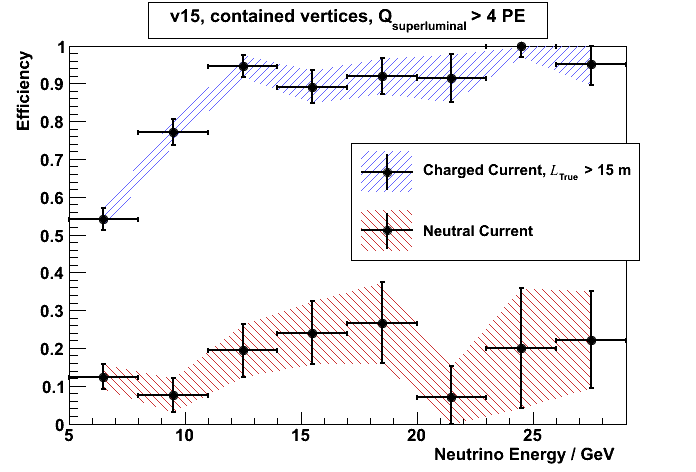
\includegraphics[width=0.4\textwidth]{figures/ExampleFigure.png}
\caption[Caption to go in list of figures]{Caption to go underneath figure}
\label{fig:example_figure}
\end{figure}

\section{Section Name 2}
Blah blah blah Here's an example of a table: see Table~\ref{tab:best_values}.

\begin{table}[H]
\centering\onehalfspacing
\vline
\begin{tabular}{c c c}
\hline
\textbf{Parameter} & \vline & \textbf{Current Best Value}\\
\hline
$\Delta m^2_{21}$ & \vline & $7.50^{+0.19}_{-0.20} \times 10^{-3}\;\mathrm{eV}^2$\\
$|\Delta m^2_{32}|$ & \vline & $2.32^{+0.12}_{-0.08} \times 10^{-5}\;\mathrm{eV}^2$\\
$\sin^2{(\theta_{12})}$ & \vline & $0.857^{+0.023}_{-0.025}$\\
$\sin^2{(2\theta_{23})}$ & \vline & $>0.95$\\
$\sin^2{(\theta_{13})}$ & \vline &  $0.098\pm 0.013$\\
\hline\end{tabular}\vline
\captionsetup{width=0.86\textwidth}
\caption[Name of table for list of tables]{Name of table for caption above table}
\label{tab:best_values}
\end{table}

Here's an example of an equation and some math:
\begin{equation}
  U = \begin{pmatrix} c_{12}c_{13} & s_{12}c_{13} & s_{13}e^{i\delta}\\
    -s_{12}c_{23} - c_{12}s_{23}s_{13}e^{i\delta} & c_{12}c_{23} - s_{12}s_{23}s_{13}e^{i\delta} & s_{23}c_{13}\\
    s_{12}s_{23} - c_{12}c_{23}s_{13}e^{i\delta} & -c_{12}s_{12} - s_{12}c_{23}s_{13}e^{i\delta} & c_{23}c_{13}
  \end{pmatrix},
\end{equation}
with $c_{ij} = \cos{\theta_{ij}}$ and $s_{ij} = \sin{\theta_{ij}}$.

Here's an example citation: \citep{PDG}.
%%%%%%%%%%%%%%%%%%%%%%%%%%%%%%%%%%%%%%%%%%%%%%%%
% chapter2.tex                                 %
% Contains formatting and content of chapter 2 %
%%%%%%%%%%%%%%%%%%%%%%%%%%%%%%%%%%%%%%%%%%%%%%%%
\chapter{Problem Statement}
\newpage
 % add more of these as necessary
%%%%%%%%%%%%%%%%%%%%%%%%%%%%%%%%%%%%%%%%%%%%%%%%
% chapter3.tex                                 %
% Contains formatting and content of chapter 3 %
%%%%%%%%%%%%%%%%%%%%%%%%%%%%%%%%%%%%%%%%%%%%%%%%
\chapter{Methodology}
\newpage
%%%%%%%%%%%%%%%%%%%%%%%%%%%%%%%%%%%%%%%%%%%%%%%%
% chapter4.tex                                 %
% Contains formatting and content of chapter 4 %
%%%%%%%%%%%%%%%%%%%%%%%%%%%%%%%%%%%%%%%%%%%%%%%%
\chapter{Results}
\newpage
%%%%%%%%%%%%%%%%%%%%%%%%%%%%%%%%%%%%%%%%%%%%%%%%
% chapter5.tex                                 %
% Contains formatting and content of chapter 5 %
%%%%%%%%%%%%%%%%%%%%%%%%%%%%%%%%%%%%%%%%%%%%%%%%
\chapter{Conclusions and Recommendations For Future Work}
\newpage
% same for the backmatter
\backmatter
%%%%%%%%%%%%%%%%%%%%%%%%%%%%%%%%%%%%%%%%%%%%%%%%%%%%%%%%%%%%%%%%%%%%%%%%%%%%%%
% bibliography.tex                                                           %
% This file gives instructions for including and formatting the bibliography %
%%%%%%%%%%%%%%%%%%%%%%%%%%%%%%%%%%%%%%%%%%%%%%%%%%%%%%%%%%%%%%%%%%%%%%%%%%%%%%

\addcontentsline{toc}{chapter}{Reference} % adds the bibliography to the table of contents
\bibliography{backmatter/ugrad_thesis.bib} % this includes the bibliography
\bibliographystyle{unsrt} % change this to change the style of the bibliography and citations


\end{document}

